\documentclass[11pt]{article}
\usepackage[margin=1in]{geometry}
\usepackage{tikz}
\usetikzlibrary{arrows.meta,positioning,fit,backgrounds,calc,shapes.geometric}
\usepackage{amsmath,amssymb,booktabs,longtable,array,microtype,rotating}
\usepackage[hidelinks]{hyperref}
\usepackage{caption}
\captionsetup{font=small,labelfont=bf}
% First argument is a machine-checkable node ID; all drawn variables have an entry.
\newcommand{\entry}[5]{\ensuremath{#2} & #3 & #4 & #5 \\[5pt]}
\title{A simplified Bayesian model of process evidence and burden}
\author{Regulatory complexity programme}
\date{September 16, 2026}
\begin{document}
\maketitle

\section{The object of inference}
The object is a distribution over plausible operating processes, not a vote
over documents and not a duration estimate with extra labels. We separate
uncertainty about the process from variation between cases and uncertainty in
the evidence. Timing is central: calendar elapsed time, applicant work-hours,
and agency work-hours are different quantities with different likelihoods.
Unmeasured labor is unknown, not zero and not a conversion from waiting days.

The unit is a jurisdiction $j$, programme $p$, and version $v$. These indices
are suppressed inside the diagram. The pilot fits one static version; the
version index does not imply that a temporal transition model is implemented.
The step inventory includes back-office activities and standing obligations;
the route model determines which of them a particular case encounters.
An activity is a coherent actor's work operation with a meaningful output, not a
sentence or an automatic legal state through inaction. Repetition is indexed by
$r$ and does not create a new activity type.

\begin{figure}[p]
\centering
\resizebox{.92\textwidth}{!}{% Simplified process-evidence model. See generative_model.tex for every symbol.
% White = latent; shaded = observed; double outline = deterministic derived value;
% dashed outline = shared parameter. All arrows are generative dependencies.
% Rework cycles live INSIDE G/R, never as cycles in this Bayesian DAG.
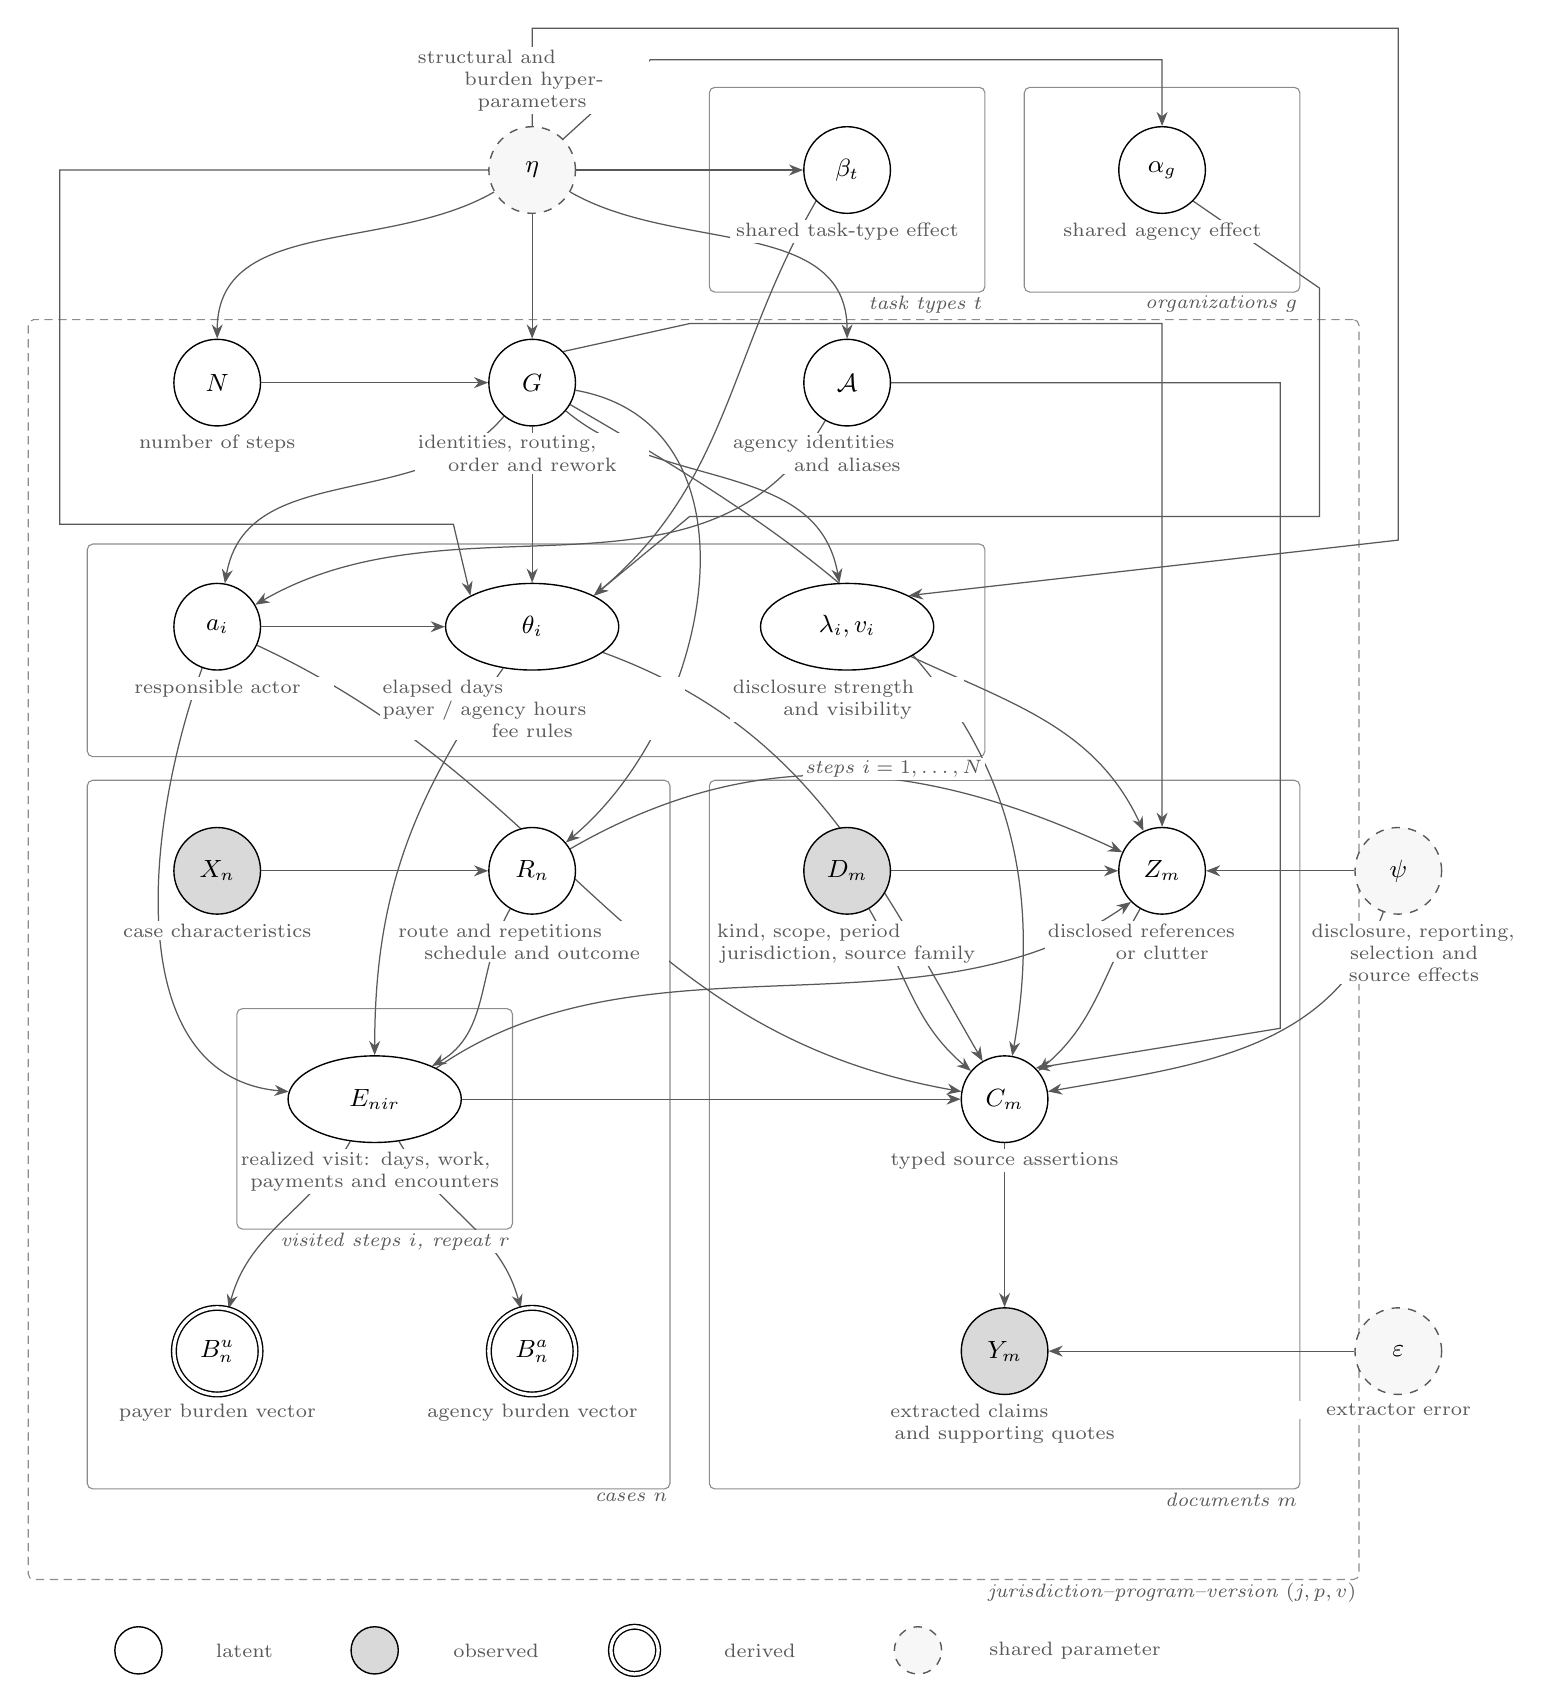
\begin{tikzpicture}[
  x=1cm,y=1cm,
  latent/.style={circle,draw=black,line width=.5pt,fill=white,
    minimum size=11mm,inner sep=1pt,font=\small},
  obs/.style={latent,fill=black!15},
  hyper/.style={latent,dashed,draw=black!65,fill=black!3},
  wide/.style={latent,ellipse,minimum width=22mm,minimum height=11mm},
  derived/.style={latent,double,double distance=1.2pt},
  lab/.style={font=\scriptsize,text=black!65,fill=white,text width=29mm,align=center,inner sep=1pt},
  plate/.style={draw=black!45,rounded corners=2pt,inner sep=2.5mm,line width=.4pt},
  outer/.style={plate,densely dashed,inner sep=9mm},
  ptag/.style={font=\scriptsize\itshape,text=black!65,fill=white,inner sep=1pt},
  ed/.style={-{Stealth[length=1.8mm,width=1.4mm]},draw=black!65,line width=.45pt}
]
\pgfdeclarelayer{edges}
\pgfsetlayers{background,edges,main}
% Program-level state. Indices (jurisdiction, program, version) suppressed.
\node[hyper] (eta) at (4.0,2.7) {$\eta$};
\node[lab,above=4pt of eta] {structural and\newline burden hyperparameters};
\node[latent] (beta) at (8.0,2.7) {$\beta_t$};
\node[lab,below=2pt of beta] {shared task-type effect};
\node[latent] (alpha) at (12.0,2.7) {$\alpha_g$};
\node[lab,below=2pt of alpha] {shared agency effect};
\node[latent] (N) at (0,0) {$N$};
\node[lab,below=2pt of N] {number of steps};
\node[latent] (G) at (4.0,0) {$G$};
\node[lab,below=2pt of G] {identities, routing,\newline order and rework};
\node[latent] (A) at (8.0,0) {$\mathcal A$};
\node[lab,below=2pt of A] {agency identities\newline and aliases};

% Step plate.
\node[latent] (a) at (0,-3.1) {$a_i$};
\node[lab,below=2pt of a] {responsible actor};
\node[wide] (theta) at (4.0,-3.1) {$\theta_i$};
\node[lab,below=2pt of theta,text width=38mm] {elapsed days\newline payer / agency hours\newline fee rules};
\node[wide] (lambda) at (8.0,-3.1) {$\lambda_i,v_i$};
\node[lab,below=2pt of lambda] {disclosure strength\newline and visibility};

% Case plate and the nested visit plate: repeats have an explicit index r.
\node[obs] (X) at (0,-6.2) {$X_n$};
\node[lab,below=2pt of X] {case characteristics};
\node[latent] (R) at (4.0,-6.2) {$R_n$};
\node[lab,below=2pt of R,text width=34mm] {route and repetitions\newline schedule and outcome};
\node[wide] (E) at (2.0,-9.1) {$E_{nir}$};
\node[lab,below=2pt of E,text width=34mm] {realized visit: days, work,\newline payments and encounters};
\node[derived] (Bu) at (0,-12.3) {$B_n^u$};
\node[lab,below=2pt of Bu] {payer burden vector};
\node[derived] (Ba) at (4.0,-12.3) {$B_n^a$};
\node[lab,below=2pt of Ba] {agency burden vector};

% Document plate. True assertions are latent; only extraction is observed.
\node[obs] (D) at (8.0,-6.2) {$D_m$};
\node[lab,below=2pt of D,text width=33mm] {kind, scope, period\newline jurisdiction, source family};
\node[latent] (Z) at (12.0,-6.2) {$Z_m$};
\node[lab,below=2pt of Z] {disclosed references\newline or clutter};
\node[latent] (C) at (10.0,-9.1) {$C_m$};
\node[lab,below=2pt of C] {typed source assertions};
\node[obs] (Y) at (10.0,-12.3) {$Y_m$};
\node[lab,below=2pt of Y] {extracted claims\newline and supporting quotes};
\node[hyper] (psi) at (15.0,-6.2) {$\psi$};
\node[lab,below=2pt of psi,text width=26mm,xshift=2mm] {disclosure, reporting,\newline selection and source effects};
\node[hyper] (epsilon) at (15.0,-12.3) {$\varepsilon$};
\node[lab,below=2pt of epsilon] {extractor error};

% Plates use coordinates to leave labels clear of their borders.
\begin{scope}[on background layer]
  \node[plate,fit={(6.5,3.5) (9.5,1.4)}] (Ptask) {};
  \node[plate,fit={(10.5,3.5) (13.5,1.4)}] (Pagency) {};
  \node[plate,fit={(-1.4,-2.3) (9.5,-4.5)}] (Pstep) {};
  \node[plate,fit={(.5,-8.2) (3.5,-10.5)}] (Pvisit) {};
  \node[plate,fit={(-1.4,-5.3) (5.5,-13.8)}] (Pcase) {};
  \node[plate,fit={(6.5,-5.3) (13.5,-13.8)}] (Pdoc) {};
  \node[outer,fit={(-1.5,-.1) (13.6,-14.3)}] (Pprogram) {};
\end{scope}
\node[ptag,anchor=north east] at (Ptask.south east) {task types $t$};
\node[ptag,anchor=north east] at (Pagency.south east) {organizations $g$};
\node[ptag,anchor=north east] at (Pstep.south east) {steps $i=1,\ldots,N$};
\node[ptag,anchor=north east] at (Pvisit.south east) {visited steps $i$, repeat $r$};
\node[ptag,anchor=north east] at (Pcase.south east) {cases $n$};
\node[ptag,anchor=north east] at (Pdoc.south east) {documents $m$};
\node[ptag,anchor=north east] at (Pprogram.south east) {jurisdiction--program--version $(j,p,v)$};

% All parents agree with the factorization in generative_model.tex.
% Put sticks behind labels and nodes so text is never struck through.
\begin{pgfonlayer}{edges}
\draw[ed] (eta) to[out=210,in=90] (N);
\draw[ed] (eta) -- (G);
\draw[ed] (eta) to[out=330,in=90] (A);
\draw[ed] (eta) -- (beta);
\draw[ed] (eta.north east) -- (5.5,4.1) -- (12,4.1) -- (alpha.north);
\draw[ed] (beta.south west) to[out=240,in=40] (theta.north east);
\draw[ed] (alpha.south east) -- (14,1.2) -- (14,-1.7) -- (6,-1.7) -- (theta.north east);
\draw[ed] (a) -- (theta);
\draw[ed] (eta) -- (-2,2.7) -- (-2,-1.8) -- (3,-1.8) -- (theta.north west);
\draw[ed] (N) -- (G);
\draw[ed] (G) to[out=230,in=80] (a);
\draw[ed] (A) to[out=240,in=30] (a);
\draw[ed] (G) -- (theta);
\draw[ed] (eta.north) -- (4,4.5) -- (15,4.5) -- (15,-2.0) -- (lambda.north east);
\draw[ed] (G) to[out=320,in=100] (lambda);
\draw[ed] (G) to[out=350,in=40,looseness=1.1] (R);
\draw[ed] (X) -- (R);
\draw[ed] (R) to[out=240,in=30] (E);
\draw[ed] (a) to[out=250,in=175] (E);
\draw[ed] (theta) to[out=235,in=90] (E);
\draw[ed] (E) to[out=240,in=75] (Bu);
\draw[ed] (E) to[out=300,in=105] (Ba);
\draw[ed] (G.north east) -- (6,.75) -- (12,.75) -- (Z.north);
\draw[ed] (lambda) to[out=335,in=115] (Z);
\draw[ed] (D) -- (Z);
\draw[ed] (psi) -- (Z);
\draw[ed] (R) to[out=30,in=155] (Z);
\draw[ed] (E.north east) to[out=35,in=215,looseness=.9] (Z.south west);
\draw[ed] (Z) to[out=240,in=40] (C);
\draw[ed] (D) to[out=300,in=140] (C);
\draw[ed] (psi) to[out=250,in=10] (C);
\draw[ed] (theta) to[out=340,in=120] (C);
\draw[ed] (a) to[out=335,in=170,looseness=1.05] (C);
\draw[ed] (G) to[out=330,in=80,looseness=1.1] (C);
\draw[ed] (A) -- (13.5,0) -- (13.5,-8.2) -- (C.north east);
\draw[ed] (E) -- (C);
\draw[ed] (C) -- (Y);
\draw[ed] (epsilon) -- (Y);
\end{pgfonlayer}

% Legend (not model variables).
\node[latent,minimum size=6mm] (legendlatent) at (-1,-16.1) {};
\node[lab,anchor=west,text width=17mm] at (-.55,-16.1) {latent};
\node[obs,minimum size=6mm] (legendobs) at (2,-16.1) {};
\node[lab,anchor=west,text width=21mm] at (2.45,-16.1) {observed};
\node[derived,minimum size=6mm] (legendderived) at (5.3,-16.1) {};
\node[lab,anchor=west,text width=22mm] at (5.75,-16.1) {derived};
\node[hyper,minimum size=6mm] (legendhyper) at (8.9,-16.1) {};
\node[lab,anchor=west,text width=30mm] at (9.35,-16.1) {shared parameter};
\end{tikzpicture}
}
\caption{\textbf{Uncertain processes, selective evidence, and two sides of burden.}
For one jurisdiction--program--version, $N$ is the finite number of steps,
$G$ their identities and routing, and $\mathcal A$ the agency entities and aliases.
Step $i$ has actor $a_i$, burden parameters $\theta_i$, disclosure strength
$\lambda_i$, and visibility $v_i$. Shared agency effects $\alpha_g$ and task-type
effects $\beta_t$, governed by hyperparameters $\eta$, pool information across
activities and programs. Actor $a_i$ selects the applicable agency effect.
Case characteristics $X_n$ select a route and outcome $R_n$; each step visit
$E_{nir}$ realizes elapsed days, applicant work-hours, agency work-hours, fees and
encounters. Payer burden $B_n^u$ and agency burden $B_n^a$ are deterministic,
vector-valued summaries of those visits and their schedule. Document metadata
$D_m$ and reporting parameters $\psi$ govern which steps or segments $Z_m$ are
disclosed and what typed assertions $C_m$ the source makes. The $E\to Z_m$ edge
allows long or burdensome cases to be reported disproportionately. Extractor error
$\varepsilon$ connects those latent assertions to the observed package $Y_m$.
An official median is informed directly by $\theta_i$; a case account by
$E_{nir}$. Elapsed time is never equated with hands-on labor. The figure specifies
the target model; the accompanying glossary distinguishes implemented pilot
components, fixed assumptions, and unimplemented extensions.}
\label{fig:plate-simplified}

\end{figure}

\section{Target joint distribution}
Condition on available case metadata $X=\{X_n\}$ and document metadata
$D=\{D_m\}$. Missing metadata must be represented as latent rather than silently
filled. Bundled nodes collect related quantities without asserting their
independence. Write $a=\{a_i\}$, $\theta=\{\theta_i\}$ and
$\Lambda=\{(\lambda_i,v_i)\}$. The arrows correspond to
\begin{align*}
p(\cdot\mid X,D)={}&p(\eta)p(\alpha\mid\eta)p(\beta\mid\eta)p(\psi)p(\varepsilon)
 p(N\mid\eta)p(\mathcal A\mid\eta)p(G\mid N,\eta)\\
&\times\prod_{i=1}^{N}p(a_i\mid\mathcal A,G)
 p(\theta_i\mid G,a_i,\alpha,\beta,\eta)p(\lambda_i,v_i\mid G,\eta)\\
&\times\prod_n p(R_n\mid G,X_n)
 p(E_n\mid R_n,a,\theta)\,
 \delta_{f_u(E_n)}(B_n^u)\,
 \delta_{f_a(E_n)}(B_n^a)\\
&\times\prod_m p(Z_m\mid G,\Lambda,D_m,\psi,R,E)
 p(C_m\mid Z_m,D_m,\psi,G,\mathcal A,a,\theta,E)
 p(Y_m\mid C_m,\varepsilon).
\end{align*}
Here $R_n$ includes case characteristics needed to generate visits, and $E_n$
is the collection of visit variables $E_{nir}$, including scheduling and actor
metadata needed for burden accounting. $E,R$ denote the
collections of cases potentially described by sources. For non-case sources
the case-specific parents are inactive. $\delta_{f(x)}$ is a point mass at the
deterministic function $f(x)$, not another stochastic burden model. Shared
source effects in $\psi$ represent dependence within a source family. Copies
must also be deduplicated or linked to a shared underlying claim; a common
reporting offset alone does not remove duplicate measurement noise. The
$E\to Z_m$ edge permits duration-dependent reporting (for example,
long delays being more likely to be mentioned); outcome-dependent reporting also
uses $R$. Neither selection mechanism is identified in the V4 fit.
We condition on the acquired corpus; modeling the search/retrieval
policy and nonpublication is an extension, not an assumption of random sampling.

\section{Every term in the diagram}
\small
\setlength{\tabcolsep}{4pt}
\begin{longtable}{@{}>{\raggedright\arraybackslash}p{1.6cm}>{\raggedright\arraybackslash}p{1.5cm}>{\raggedright\arraybackslash}p{6.2cm}>{\raggedright\arraybackslash}p{5.7cm}@{}}
\toprule Symbol & Type & Definition and support & V4 status / evidence \\
\midrule\endfirsthead
\toprule Symbol & Type & Definition and support & V4 status / evidence \\
\midrule\endhead
\bottomrule\endfoot
\entry{eta}{\eta}{Shared}{Structural and burden hyperparameters: finite count,
agency/task heterogeneity and duration/effort distributions.}{V4 learns the global
log-duration location, agency/task/step scales and case spread. Hyperpriors and
unidentified coverage assumptions remain explicit; no held-out truth is fitted.}
\entry{alpha}{\alpha_g}{Latent}{Organization $g$'s task-adjusted log-duration effect,
shared across activities and programs. $g$ indexes canonical organization identities;
actor $a_i$ selects the corresponding effect.}{Jointly learned in V4. Task reports
inform their agency and other tasks at that agency. Work-hour effects are fitted
separately when observed; elapsed delay is not staff productivity.}
\entry{beta}{\beta_t}{Latent}{Task-type $t$'s log-duration effect, shared across
agencies and programs; task type is part of $G$.}{Jointly learned in V4 with agency
and activity residual effects. Multiple tasks per agency and crossed task types
are needed to disentangle these components.}
\entry{N}{N}{Latent}{Total distinct activity count, including activities with no
detected mention. Nonnegative integer.}{Represented inventory plus a sampled,
truncated geometric number of undocumented stages. This is an explicit sensitivity
prior, not learned document coverage. Distinct from repeated visits.}
\entry{G}{G}{Latent}{Finite graph: step identities, semantic operation descriptions,
applicability, precedence, alternatives, and rework links. Base precedence is a
DAG; repeat links are separate.}{Semantic inventory fixed by a source-only LLM audit.
Finite precedence completions sampled; conditional route prevalence has explicit
priors. Complex branching, repeated execution and abandonment are not fitted.}
\entry{A}{\mathcal A}{Latent}{Finite set of participating organization identities,
roles and aliases. Directories provide evidence, not a guaranteed complete roster.}{Uses
quote-supported actor roles and distinctive aliases within a jurisdiction.
Conditional on the LLM's organization mapping; no full organization hierarchy or
posterior over entirely unlisted agencies.}
\entry{a}{a_i}{Latent}{Responsible actor for step $i$, categorical over
$\mathcal A$ plus external participants. Executing and receiving roles may differ.}{Fixed
by the validated semantic interpretation in V4. Agency effects are inferred, but
uncertain actor identity and multiple responsible roles remain extensions.}
\entry{theta}{\theta_i}{Latent}{Step burden parameters: log-median $\mu_i$ and case
spread $\sigma_i$ for elapsed days; separate work-hour parameters for payer and
agency; conditional fee schedule; input, payment and encounter rules.}{Elapsed
time fitted on a grid in V3; V4 jointly samples an agency/task/step hierarchy.
Work-hour channels have separate likelihoods and priors. No staffing/queue
decomposition is inferred. V4 retains fees in the evidence ledger.}
\entry{lambda}{\lambda_i,v_i}{Latent}{Step disclosure intensity $\lambda_i>0$ and
visibility stratum $v_i\in\{\mathrm{public},\mathrm{internal}\}$. Together with
document-kind exposure these generate mention counts.}{Target only in V4: coverage
and disclosure selection are not identified. V3 used an assumed Gamma intensity
and visibility mixture; V4 reports count-prior sensitivity explicitly.}
\entry{X}{X_n}{Observed}{Case attributes: payer/project type, relevant conditions,
and start period. Unknown attributes would be latent.}{Quote-supported case/cohort
inclusions, exclusions and directly observed work constrain routes. Other conditional
frequencies use uncalibrated priors; no representative cohort model is claimed.}
\entry{R}{R_n}{Latent}{Case route and outcome, including visited steps, correction
rounds, and precedence/parallel scheduling. A route can end in approval, denial
or abandonment.}{V4 fits DAG schedules and conditional operations. Multiple
decision operations are alternative endpoints. Observed outcomes condition cases/cohorts;
unknown population proportions have a logistic-Normal prior. Repeated visits and
abandonment are not fitted.}
\entry{E}{E_{nir}}{Latent}{Visit $r$ to step $i$ by case $n$: begin/end times,
elapsed days, payer and agency labor-hours, cash transaction, and encounter
identity. Includes actor identity for attribution.}{Actual latent case durations
are jointly fitted to the same case's totals and breakdowns. Population durations
are integrated by Sobol quadrature. Labor is fitted separately when measured;
transaction and repeated-visit accounting remains outside V4.}
\entry{Bu}{B_n^u}{Derived}{Payer vector: calendar delay, hands-on hours,
out-of-pocket payments, trips/contacts, repeat submissions and sensitive
disclosures. $u$ means user/payer.}{V4 emits elapsed time and modeled operation
counts; work-hours when observed. Fees, trips, sensitive disclosures, and repeat
visits are not claimed as fitted burden totals.}
\entry{Ba}{B_n^a}{Derived}{Agency vector: agency work-hours by organization,
task executions, handoffs/rework and operating cost where measured. $a$ means
agency, not the actor variable $a_i$.}{Represented agency operations and organization
counts emitted. A separate staff-hours likelihood uses reported effort (including
a J1/S01 two-hour cost-study estimate). Agency-specific labor allocations are
weakly identified. Operating costs and standing overhead are not fitted.}
\entry{D}{D_m}{Observed}{Document metadata: kind, jurisdiction, relevant interval,
publication date, timing scope, statistic type, and known source family.}{Known
fields retained; missing scope is flagged. Explicit historical/hypothetical reports
are excluded from current-process fitting, not dynamically modeled. Publication
date alone does not identify the period measured.}
\entry{Z}{Z_m}{Latent}{Which steps or segments document $m$ mentions and the
mapping of each assertion to them. Empty/spurious references are allowed.}{V4 fixes
step/segment mappings from quote-validated LLM interpretation. Granularity audits
preserve every original mapping. Entirely undisclosed stages remain prior-sensitive.}
\entry{C}{C_m}{Latent}{What the source actually asserts: existence, actor, order,
fees, individual waits, reported summaries, effort and normative rules. This is
not automatically a correct claim about the process.}{Typed interval likelihoods
fit realized waits and summaries, with shared source offsets and a contamination
component. Executed segments, selected cohorts and clock-start milestones have
explicit semantics. Raw-text interpretation error is not calibrated; caps/targets
never enter realized-duration likelihoods.}
\entry{Y}{Y_m}{Observed}{Extracted per-document structured claims with supporting
quotes and provenance. This is the instrument output, not a gold process.}{V4 uses
public-document interpretation and the backward-compatible process-evidence/3 contract.
No solver answers, truth processes, ceilings, or hidden specifications enter fitting.}
\entry{psi}{\psi}{Shared}{Disclosure exposure by kind and visibility; source
fidelity and bias; case-report selection; shared source-family effects.}{Shared
source-family timing offsets jointly learned; exact known copies deduplicated.
The offset prior is sensitivity-tested. Complaint selection, unknown copying,
document exposure and domain-transfer calibration remain unidentified.}
\entry{epsilon}{\varepsilon}{Shared}{Extractor sensitivity, false positives,
field confusion and numeric interpretation errors, conditional on field/kind.}{Not
separately identified from source error: quote validation is not semantic
calibration. Robust reporting error does not replace audited extraction labels.}
\end{longtable}
\normalsize

\section{Timing and two burden channels}
Elapsed duration satisfies $\log D_{nir}\sim\mathcal N(\mu_i,\sigma_i^2)$ in the
first version. Work-hours $H_{nir}^u,H_{nir}^a$ have separate positive distributions
when observed. A reported population median informs $\mu_i$, not an individual
case draw. For a sample median based on $s$ independent log-normal cases, the
large-sample log-median variance is approximately $\pi\sigma_i^2/(2s)$, to which
reporting uncertainty must be added. Unknown $s$ does not imply a precise median.
Intervals use interval likelihoods; zero-day reports are rounded intervals.
Business days are not silently converted to calendar days. Legal caps and
service targets are retained as normative metadata, never as realized waits.

Elapsed case time follows the realized prerequisite schedule, with parallel
branches overlapping. Hands-on hours sum work events, not waiting days.
Flat fees are charged once per transaction, per-visit fees on each applicable
visit, and shared encounters are counted once. Standing agency overhead is
reported separately from per-case effort; converting it to a per-case allocation
requires workload and time-horizon assumptions.

\section{What is actually implemented}
The target joint above is \emph{not} claimed as a fully fitted model.
The historical V3 pilot uses a modular (cut) posterior:
structure and actor inference from name/relationship evidence; typed timing
and fee inference conditional on each structure; then case simulation. Timing
does not feed back into entity resolution. Disclosure, source reliability and
extractor error are not jointly identified. A posterior under these assumptions
is not a demonstration of calibration.

V4 replaces the timing cut with joint inference over agency/task/activity effects,
latent case durations, source offsets, finite schedule completions and undocumented
stage counts. Both total and step reports observe the same latent case. Typical
and population-summary claims observe summaries of the route distribution. Thus
information can propagate upward to agencies and downward to unmeasured tasks.
Semantic entity reconciliation remains an upstream LLM instrument with a strict,
quote-validated schema; its output is not treated as an error-calibrated posterior.
Source-only context and clock audits keep selected-cohort reports separate from
unconditional claims, share known outcomes across a case, and preserve segment
timing outside the initial route. A clock beginning after an operation excludes
that completed operation's duration. None of these audits sees benchmark truth.
The glossary describes V4 status against the broader target model. Exact scope,
diagnostics and residual limitations are documented in
\texttt{docs/2026-09-16-bayesian-process-v4.md}.

The V4 elapsed hierarchy is
\[
 \mu_i=m+\alpha_{a_i}+\beta_{t(i)}+\gamma_{p(i)}+\delta_i,
 \qquad \log D_{ni}=\mu_i+c_n+\sigma z_{ni}.
\]
Here $m$ is the global log-duration location; $t(i)$ and $p(i)$ identify task type
and program; $\gamma_p$ is a program effect; $\delta_i$ is an activity residual;
$c_n$ is a shared case shock; and $z_{ni}\sim\mathcal N(0,1)$ is independent
case-step variation. These are components of the bundled $\eta,\theta_i,E_{nir}$
nodes, not additional unlabeled diagram nodes. Conditional scale priors and all
likelihood approximations are explicit in the implementation document.

The count model explicitly distinguishes detected steps from undisclosed steps.
Burden for wholly undisclosed steps is weakly identified: V4 gives those stages
explicit prior-predictive durations and reports sensitivity, rather than treating
them as zero-duration additions. Agency counts remain conditional on resolved
labels; the number of completely unlisted agencies is not inferred.
The implementation does not turn these limits into invented precision.

\section{Evaluation and scoring correction}
The historical V3 pilot used ten cached document extractions for W1/J1/S03. Gold was loaded
only after posterior files have been written. It is not an equal-information
head-to-head with the one-pass LLM: the legacy cache omits process-level claims.
The runner records seeds, configuration, source hashes, posterior draws, count
sensitivity and basic chain diagnostics. It also rescores eight saved oracle
and three saved search runs, preserving the original scores.

The scorer now reads \texttt{process\_timing.median\_days}; it no longer substitutes
a sum of step medians for missing end-to-end predictions. Across the saved runs,
the corrected median multiplicative end-to-end error is approximately $1.075$
for oracle documents and $1.321$ for search, instead of $1.545$ and $2.387$.
Those are point-prediction measurements, not posterior calibration results.
The V4 protocol and subsequent results are documented separately in
\texttt{docs/2026-09-16-bayesian-process-v4-protocol.md} and
\texttt{docs/2026-09-16-bayesian-process-v4-results.md}. No benchmark victory is assumed here.
\end{document}
